\section*{Preliminaries}
\label{sec.prelim}

This section presents preliminaries on networks, the clustering algorithm HLC,
and the linear regression technique LASSO.

\subsection*{Co-expression network}

Consider a network as an undirected graph $G=(V,E)$ where
${V=\{v_1,v_2,\ldots,v_{n}\}}$ is a set of $n$ \textit{vertices} (or
\textit{nodes}) and ${E=\{e_1,e_2,\ldots,e_q\}}$ is a set of $q$
\textit{edges} (or \textit{links}) that connect vertices. In a
co-expression network of genes, each node corresponds to a gene, and
a link indicates similar expression pattern between two genes.
The network can be represented by an adjacency matrix $A
\in \{0,1\}^{n \times n}$ that is symmetric. A matrix entry in 
positions $(v_i,v_j)$ and $(v_j,v_i)$ is equal to $1$ whenever there is an edge
connecting vertices $v_i$ and $v_j$, and equal to $0$
otherwise. Co-expression networks are of biological interest because
adjacent nodes in the network represent co-expressed genes that are
usually controlled by the same transcriptional regulatory pathway,
functionally related, or members of the same pathway or metabolic
complex~\cite{FIONDA2019915}.


\subsection*{Hierarchical Link Clustering}

The Hierarchical Link Clustering (HLC) algorithm partitions
groups of links (rather than nodes), each node inherits all
memberships of its links and can belong to multiple, overlapping
communities~\cite{ahn2010link}. More specifically, HLC evaluates the similarity 
between links if they share a particular node.
Consider a pair of links $e_{ik}$ and $e_{jk}$, which are adjacent to node $k$.
The similarity between $e_{ik}$ and $e_{jk}$ is defined based on the Jaccard index as
%
\begin{equation}\label{eq:jaccard}
  S(e_{ik},e_{jk}) = \frac{\vert \ \eta(i) \cap \eta(j) \ \vert}{\vert \ \eta(i) \cup \eta(j) \ \vert},
\end{equation}
%
where $\eta(i)$ denotes the set containing node $i$ and its
neighbors. The algorithm uses single-linkage hierarchical clustering
to build a dendrogram in which each leaf is a link from the
network, and branches represent link communities. 
%Hierarchical
%clustering algorithm repeatedly merge groups until all elements are
%members of a single cluster.
\vspace{0.5cm}

The threshold where to cut the dendogram is defined
based on the average density of links inside communities (partition density).
For $G=(V,E)$ and a partition of the links into $c$ subsets, the partition density is computed as

\begin{equation}
D = \frac{2}{\vert E \vert} \sum_c \vert E_c \vert \frac{\vert E_c \vert - \vert V_c \vert + 1 }{(\vert V_c \vert -1)(\vert V_c \vert -2)}
\end{equation}

Note that in most cases, the partition density $D$ has a single
global maximum along the dendrogram. 
If the dendogram is cut at the top, then $D$ represents the
average link density of a single
giant community.  If the dendogram is cut at the
bottom, then most communities consists of a single
link. In other words, note that $D = 1$ when every community
is a clique and $D = 0$ when each community is a
tree. If a community is less dense than a tree (i.e., when the
community subgraph has disconnected components), then such a community
contributes negatively to $D$, which can take negative values. The
minimum density inside a community is $-2/3$, given by one community
of two disconnected edges. Since $D$ is the average of the
intra-community density, there is a lower bound of $-2/3$ for
$D$. By computing $D$ at each level of the dendrogram, 
the level that maximizes partition density can be found 
(nonetheless meaningful
structure could exist above or below the threshold).

% figure 0
\begin{figure}[htbp]
  \centering
    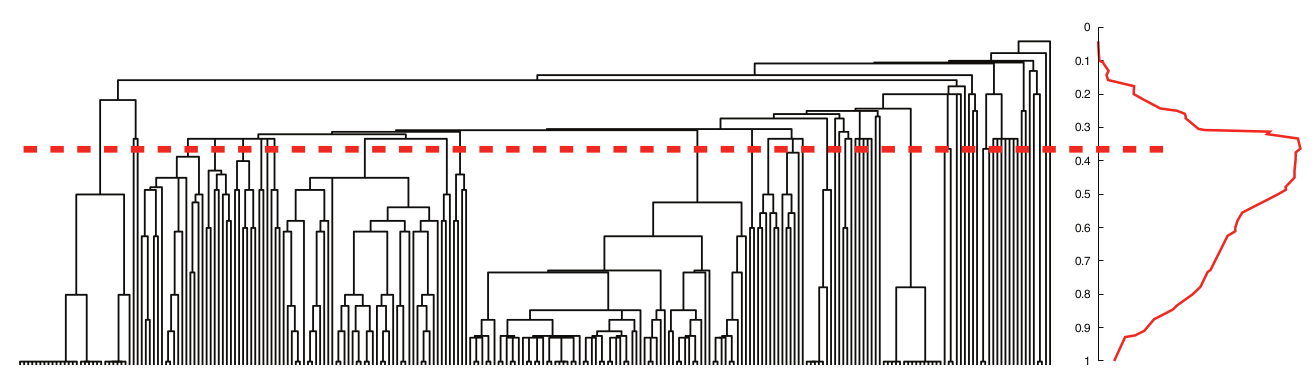
\includegraphics[clip,width=0.96\textwidth]{figures/figure0.png}
  \caption[Example of a full link dendrogram (left) and partition density (right)]%
  {Example of a full link dendrogram (left) and partition density (right), borrowed from~\cite{ahn2010link}.}
  \label{fig:hlc_density}
\end{figure}

The output of
cutting is a set of node clusters, where each node can participate in
multiple communities.

\subsection*{Least Absolute Shrinkage Selector Operator (LASSO)}

LASSO is a
regularized linear regression technique. By combining a regression
model with a procedure of contraction of some parameters towards $0$,
LASSO imposes a restriction (or a penalty) on
regression coefficients. In other words, LASSO solves the least
squares problem with restriction on the $ L_1$-norm of the coefficient
vector. In particular, the approach is especially useful in scenarios where the number
of variables $ c $ is much greater than the number of
samples $ m $ (i.e., $ c \gg m $).
\vspace{0.5cm}

Consider a dataset of $m$ samples, consisting each
of $c$ covariates and a single outcome. Let $y_i$ be the outcome and
$x_i := (x_{i1},...,x_{ic})$ be the covariate vector for the $i$-th
sample. The objective of LASSO is to solve
%
\begin{equation}
\min \left\lbrace\sum_{i=1}^{m}{\left( y_i-\sum_{j=1}^c{\beta_j
    x_{ij}}\right)^2} \right\rbrace \quad , \quad \textrm{subject to}
\quad \sum_{j=1}^c\abs{\beta_j}\leq s.
\end{equation}

where $s$ is the regularization penalty. 
Equivalently, in the Lagrangian form, LASSO minimizes

\begin{equation}
  \sum_{i=1}^{p}{\left( y_i-\sum_{j=1}^c{\beta_j x_{ij}}\right)^2} +
  \lambda \sum_{j=1}^c\abs{\beta_j}
\end{equation}
%
where $\lambda \geq 0$ is the
corresponding Lagrange multiplier. Since the value of the regularization
parameter $\lambda$
determines the degree of penalty and the accuracy of the model,
cross-validation is used to select the
regularization parameter that minimizes the
mean-squared error.
